\documentclass[letterpaper, 10pt]{article}
\usepackage[OE]{express}
\usepackage{multirow}
\usepackage{graphicx}
\usepackage{subfigure}
\usepackage{cite}
\usepackage{soul}

\begin{document}
\title{Silica-based integrated 1$\times$4 polarization beam splitter module for free-space BB84 quantum key distribution}
\author{Joong-Seon Choe, Heasin Ko, Byung-Seok Choi, Kap-Joong Kim, and Chun Ju Youn}
\address{Electronics and Telecommunications Research Institute, Daejeon 34129, Korea}
\email{jschoe@etri.re.kr}
%\thanks{Joong-Seon Choe is with ETRI.}
%\maketitle
\begin{abstract}
% 편광기반 BB84 프로토콜 기반의 QKD에 사용하기 위해 실리카 PLC 기술로 집적형 편광 분할/결합기 모듈을 개발했다.
We have developed an integrated polarization beam splitter (PBS) module with silica planar lightwave circuit technology for use in BB84 quantum key distribution (QKD).
% 4개의 편광에 대해 동작시키기 위해 반파장판을 삽입하였으며, 모듈의 편광소광비와 삽입손실은 각각 ___ dB와 ___ dB였다.
The PBS module was designed to operate on four linear polarizations of horizontal/vertical/diagonal/antidiagonal direction, and showed the minimum polarization extinction ratio of 17.6 dB.
%The excess optical loss and The minimum polarization extinction ratio were \underline{4.59} dB and \underline{17.6 dB}, respectively.
% 무선양자암호 테스트베드에 장착하였을 때 QBER과 sifted key rate은 까각 ___%와 ___kbps롤 보였다.
When the module was loaded on the free-space BB84 QKD test-bed, quantum bit error rate and sifted key rate  were 2.81\% and 415 kbps at clock rate of 100 MHz, respectively.
\end{abstract}

\ocis{(260.5430) Polarization; (230.5440)   Polarization-selective devices; (060.5565) Quantum Communications; (230.7390) Waveguides, planar }

\bibliographystyle{osajnl}
% \begin{thebibliography}{1}
% \newcommand{\enquote}[1]{``#1''}
% \expandafter\ifx\csname url\endcsname\relax
%   \def\url#1{\texttt{#1}}\fi
% \expandafter\ifx\csname urlprefix\endcsname\relax\def\urlprefix{URL }\fi
% \providecommand{\eprint}[2][]{\url{#2}}

\bibliography{jschoe}
% \end{thebibliography}

\section{Introduction}
%최근에 통신 보안에 대한 이슈가 부각되면서 양자암호통신에 대해 많은 연구가 이루어지고 있다.
Many researches have been conducted for quantum communication as security solution is one of the main issues in communication technology \cite{Bennett:1984is, Ekert:1991kl,Ko:2017cs}.
%양자 암호 통신을 위한 여러 프로토콜들 중 최초로 제안된 BB84는 가장 많이 연구되어 오고 있다.
Since Bennett and Brassard proposed BB84 protocol for secure key distribution, it has widely been chosen for quantum key distribution (QKD) \cite{Bennett:1984is}.
% BB84를 구현하기 위해서 직교하지 않는 두 베이시스 셋을 구성하며 그 수단으로 주로 편광 또는 위상을 사용한다.
Implementation of BB84 requires two sets of non-orthogonal basis %that can be constructed with either polarization or phase.
% 광신호의 전달 매체는 환경에 따라서 자유공간 또는 광섬유가 사용된다.
% 자유공간 BB84 통신에서는 편광이 잘 유지가 되므로 편광으로 신호 인코딩이 가능하다.
that are usually constructed with polarization of single photon for free-space communication.
% 광섬유를 사용할 경우 광섬유가 받는 스트레인에 의해 발생하는 복굴절이 편광의 변화를 유발하므로 원래의 편광을 유지하는 것이 어려우므로 흔히 빛의 위상으로 신호를 인코딩한다.
% 자유 공간에서는 상대적으로 편광의 변화가 적으므로 편광 인코딩의 BB84 프로토콜의 사용이 용이하다.
% 편광 기반의 BB84는 HV 또는 DA 편광으로 이루어진 베이시스 중 하나를 선택하고 선택한 베이시스의 두 편광 중 하나를 선택함으로써 데이터를 인코딩하여 보내는 방식으로 암호키를 전달한다.
The polarization-based BB84 protocol encodes the data by choosing a basis of the two bases of horizontal(H)/vertical(V) or diagonal(D)/antidiagonal(A) polarization, and transmitting a single photon of a polarization from the chosen basis to generate an encryption key.
%HVDA의 네 편광 중 하나를 선택해서 보내고 수신자는 편광을 가반으로 한 많은 연구가 수행되어 왔다.
%Polarization-based BB84 generally uses single photons with horizontal (H), vertical (V), diagonal (D), and antidiagonal (A) polarization

Thus an optical part for splitting or combining the four states of polarization is essential for a polarization-based BB84 QKD, and is generally composed of two bulk polarization beam splitters (PBS), one beam splitter, and one half-wave plate (HWP) \cite{Ko:2017cs}.
%편광을 합치고 보내는 광학계는 일반적으로 벌크 광학 부품을 정렬하여 사용하는데, 양자비트에러율은 광정렬의 정확도에 크게 의존하므로 시간이 지남에 따라 발생할 수 있는 약간의 정렬 틀어짐도 시스템의 안정성을 떨어뜨리게 된다.
Although the bulk-optic components show high performances in polarization extinction ratio (PER), optical loss, and so on, the QKD system will work only when the components are installed with high alignment accuracy upon which its overall performance is strongly dependent.
%In addition, some alignment drift over time can degrade system stability even though initial alignment status results in sufficiently low QBER.
%본 연구에서는 자유공간을 통한 편광 기반의 BB84 프로토콜 양자암호통신의 구현을 위해 광도파로 소자로 구현된 편광분할기 모듈을 개발하였고 무선 양자암호통신 테스트베드에 장착하여 키 분배 실험을 수행하였다.

The need for alignment of discrete optic components can be removed if they are replaced by integrated elements on a chip
%If the optical components are replaced by integrated elements on a chip
fabricated through semiconductor processes such as photo-lithography and dry etching.
%Integration of all the components on a chip removes the alignment processes and prevents the drift of alignment over time that can degrade system stability even though initial alignment status results in sufficiently low QBER.
The chip-scale integration provides performance stability improvement as well as miniaturization of optical part in BB84 system, and can readily be implemented using waveguide-based photonic circuit technology.
PBS chips using waveguide are widely used in optical receivers for polarization-multiplexed modulation formats such as dual polarization quadrature phase shift keying (DP-QPSK), dual polarization 16 quadrature amplitude modulation (DP-16QAM), etc  \cite{Lee:2016bg,PoDong:2014kj}.
However, there has been no report on integrated PBS chip that can deal with four polarizations used in BB84 QKD.
In this study, integrated PBS module using  silica-based planar lightwave circuit (PLC) chip was fabricated for the first time for BB84 protocol, and its performance was assessed it in a free-space QKD test-bed.

\section{Fabrication}
\subsection{PBS chip}

% PBS 소자는 실리콘 기판 위에 실리카 평판형 광도파로를 이용하여 제작하였다.
PBS developed in this work is based on Mach-Zehnder interferometer (MZI) structure fabricated with silica PLC technology \cite{Kim:2012ej, Hashizume:2015ta}.
% 사용하는 파장 대역이 780 nm이므로 여기에서 단일 모드가 되며 해당 파장에서의 광섬유와 높은 광결합 효율을 가지도록 기본 도파로를 설계하였다.
The waveguide structure was chosen to support single mode and maximum mode matching with single mode fiber (SMF) at the operating wavelength of 780 nm, where Si single photon detector has high detection efficiency and atmospheric absorption is low.
% 코어와 클래드의 굴절률은 780 nm의 파장에서 각각 ___와 ___였으며 도파로 코어의 크기는 가로와 세로가 모두 4.3 um이다.
Refractive indices of core and clad material were 1.4588 and 1.4537 at 780 nm, respectively, and the dimension of waveguide core was designed as 4.3 $\mu$m $\times$ 4.3 $\mu$m.
% 마흐 젠더 간섭계 구조에서 한 쪽 arm에서 수직과 수평의 두 편광간에 180도의 retardation이 나타나도록 하고 다른 쪽 arm과는 두 편광이 모두 90도의 위상차가 존재하도록 하면 두 편광을 분리할 수 있다.
In the MZI structure, H- and V-polarizations can be separated by providing a retardance of 180$^\circ$  between the two polarizations in one arm while both the polarizations have phase difference of 90$^\circ$  between the two arms \cite{Kim:2012ej}.
% retardation을 가하기 위해 한 쪽 arm의 도파로 일부를 넓게 설계하였다. 이렇게 하면 제작 공정상에서 uniaxial strain을 받게 되어 복굴절이 발생함이 알려져 있으며, 복굴절 * 길이 * 2pi / 파장 = 2m*pi+pi 가 되는 길이로 제작하면 180도의 위상차가 되게 만들 수 있다.
A portion of the waveguide of one arm is designed to have larger width of 18.5 $\mu$m.
A wide waveguide in silica PLC is known to have birefringence  due to uniaxial strain generated in the fabrication process \cite{Okuno:1994fm}.
When the device is designed so that birefringence $\Delta n$ and length $L$ of the wide waveguide satisfy the condition $2\pi\Delta n/\lambda  = (2m+1) \pi$ with integer $m$, the phase difference between H- and V-polarization can be made to be 180$^\circ$.
% The required retardance was provided by designing part of one arm in MZI widely.
% Wide waveguide in silica PLC was known to suffer uniaxial strain and therefore birefringence occurs.
% As retardance is
%다른 한 쪽 arm의 길이도 적절히 설계하면 위의 모든 위상 조건을 만족하도록 하는 것이 가능하다.
If the length of the other arm is properly designed, it is possible to satisfy the aforementioned phase relationship.
% % TE and TM polarization can be split if they have phase difference of $\pi$ in one arm of MZI and $\pi/2$ between the two arms, as described in    .
% Part of an arm of MZI was designed to have wide width to impose retardance.
% Wide waveguide is known to result in uniaxial strain and thus birefringence occurs.
% As retardance is
% \begin{equation}
%   \Delta n_{br}L \times 2\pi / \lambda
% \end{equation},
%appropriate length can give phase difference of $\pi$..
%\subsection{P\Delta n_{br}L \times BS chip}2\pi / \lambda
%The other arm of MZI can meet above phase relation for polarization splitting with appropriate length.
%그러나, 위상 조건은 길이에 의해서 정해지나 실제로 온도의 변화에 따라서 민감하게 달라지므로 간섭계 구조를 사용할 경우 active 하게 조절하는 것이 필요하다.

The phase relationship is determined by arm length, as described above.
But actually it changes sensitively with ambient temperature around the interferometer structure.
%따라서 본 연구에서는 간섭계의 arm에 히터를 장착하여 전류로 위상을 조절할 수 있도록 했다.
Therefore, micro-heaters were deposited on the arms of MZI to actively control the phase making use of the themo-optic property of silica.

%다음 그림은 소자의 설계 도면과 제작이 완료된 칩바의 사진이다.

Figure \ref{fig:layout} shows the layout of the device.
% and photograph taken after fabrication process is completed.
The input light is split into two paths by the 3 dB splitter.
At the outputs of a 3 dB splitter are connected in parallel the two identical birefringent MZIs with 2$\times$2 multimode interference device at their outputs.
Each birefringent MZI in this device splits the input light into H- and V-polarized light.
%The input light is split into two paths by the 3 dB splitter and separated into H-and V-polarized light in each PBS.
%The PBS splits H and V while input polarization can be D or A, thus a half-wave plate is to be inserted in front of the lower PBS.
%소자의 길이는 42 mm 이고 폭은 1.2 mm 이다.
%Each device is 42 mm and 2.3 mm in length and width.
%Figure \ref{fig:device} shows layout of the device developed in this study.
\begin{figure}
  \centering
  \includegraphics[width=8cm]{./layout}
  \caption{(a) Layout of the PBS device for H/V/D/A-polarizations. 1$\times$2 splitter splits the input light into two PBSes that separate H- and V-polarization and output them to the corresponding waveguides. Lower PBS has HWP at its input so that D- or A-polarized light is converted to H- or V-polarization. (b) Schematic description of the operation of 2$\times$2 MMI. Under single port input, the two outputs show same power with relative phase difference of 90$^\circ$ (upper). If there is phase difference of 90$^\circ$ between two inputs, one output is extinguished (lower).}
  \label{fig:layout}
\end{figure}
% 입력된 빛은 1X2 splitter에서 갈라지고 각각 HV에 대한 PBS에서 편광별로 분리되어 각각의 출력으로 나가도록 되어 있다.
% 입력되는 빛은 HV 뿐만 아니라 DA 베이시스인 경우도 있으나 사각도파로로 구성된 PLC PBS에서 D와 A를 제대로 분리할 수 없다.
The input light may be in D/A-polarization basis as well as H/V-polarization basis, but D- and A-polarized light can not be properly separated in PLC PBS composed of rectangular waveguide.
% 따라서 본 연구에서는 두 MZI중 하나의 입력부에 slit을 형성하고 광축이 22.5도 기울어진 반파장 필름을 삽입하여 DA에서 HV로 편광을 바꾼 후 분리하는 방법을 취했다.
Therefore, in this study, a HWP film with its optic axis tilted by 22.5$^\circ$ was inserted at the input of the lower PBS to split D/A polarization.
Although the output of the lower MZI is annotated as D/A in Fig. \ref{fig:layout}, actual polarization of the output light is H/V.
%Therefore, in this study, a HWP film was inserted in a slit formed a slit is formed on one input of two MZIs, and a HWP film with optic axis tilted by 22.5$^\circ$ is inserted to change polarizations from DA to HV and then separated.
% 이것은 벌크 옵틱스로 꾸민 BB84 광학계에서 사용하는 방법과 동일하다.
%This is the same method used in the general BB84 system with bulk optics.
%칩바 상태에서 편광 분리 특성을 측정하기 위해 다음 그림과 같은 측정 셋업을 사용하였다.

% Measurement  of Fig. \ref{fig:setup}  was used to characterize the polarization splitting property of the device without pigtailed fiber.
% \begin{figure}
%   \centering
%   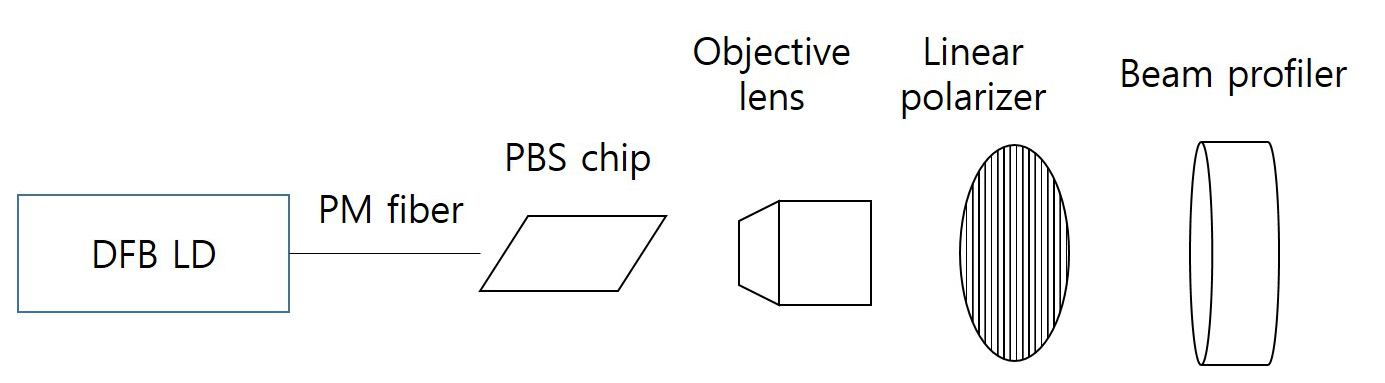
\includegraphics[width=10cm]{./setup}
%   \caption{}
%   \label{fig:setup}
% \end{figure}
% Output of a 780 nm DFB LD was delivered to a PBS chip through a polarization-maintaining fiber (PMF) whose slow axis is aligned obliquely so that incident light contains both H- and V-polarization.
% The output lights was expaned through an objective lens and observed using a beam profiler\underline{(Ophir Optronics Spiricon SP503)}.
% As the input is neither H nor V, output light has both the polarizations.
% In order to evaluate PER, a linear polarizer (LP) was placed between the objective lens and beam profiler.
% If the transmission axis of the LP is vertical, only V-polarized light is considered to be incident since the LP filters out the H-polarized light with extinction ratio exceeding 30 dB.
% This method is based on the assumption that rotation of polarization does not occur for H- and V-polarized lights.
% With polarization rotation, PER would be deteriorated when measured after the chip is fabricated to PBS module that does not contain any LP.
% As will be discussed later, however, PBS module does not show any drop of PER, which suggests the validity of the assumption.


\subsection{Half-Wave Plate Film}
%위의 파장분할기는 수직과 수평 편광의 분할 기능을 가지며, 45도와 135도의 편광에 대해서는 진행중의 회전 때문에 동작을 보장할 수 없다.
%PBS described above has function of separating H and V polarization, and does not work for D and A polarization.
%따라서 두 대각 편광을 수직 또는 수평 편광으로 바꿔주기 위한 반파장판을 도파로 중간에 삽입한 후 편광 분리 동작을 하도록 하기 위해 780 nm 파장대역용 박막 반파장판을 제작하였다.
Thin film HWP was developed for converting D/A polarization to H/V polarization that can be inserted in a slit across a waveguide.
A HWP was fabricated by imposing birefringence on a polymer film \cite{Ando:1993up}.
% 사용한 필름은 폴리카보네이트이고, 175도에서 45% 길이만큼 잡아늘여서 복굴절을 일으켰다.
Fixed at its two sides on a metal frame designed for elongation process, the film was stretched at an elevated temperature.
% 여러 조건에 대해서 필름의 연신 공정을 수행한 결과 50um 두께의 PC 필름을 40% 길이만큼 연신했을 때 반파장에 근접한 retardance를 보임을 확인했다.
Elongation process was performed for several kinds of commercial polymer film under various conditions, and it was found that 40\% elongation of 60-$\mu$m-thick polycarbonate film at 170$^\circ$C resulted in retardance near 180$^\circ$ at the wavelength of 780 $\mu$m.
The thickness of the film after process was 53 $\mu$m.
%45도/135도 편광의 입사광에 대해 사용하여야 하므로 광축을 수평면에 대해 22.5도 기울어지게 잘라내었다.
As the film was to be used for light of D/A polarization, cutting direction was selected so that the optic axis was inclined by 22.5$^\circ$ with respect to the bottom side of the film.

\subsection{PBS Module}
%우선 dicing blade로 병렬로 이어져있는 두 간섭계의 입력부 부분에 홈을 내고 반파장판 필름을 삽입하고 에폭시로 고정하였다.

Firstly, a narrow groove was formed at the input waveguides of two parallel MZIs comprising 1$\times$4 PBS with a dicing blade for the insertion of the waveplate film.
% 반파장판은 한 쪽 간섭계에만 필요하나 두 간섭계간의 거리가 가까와서 dicing blade로는 양 쪽 모두에 홈을 낼 수밖에 없다.
Waveplate is needed for only one MZI of the PBS, but the groove spans  both the MZIs because of the small separation of 500 $\mu$m, resulting in similar optical loss between the two MZIs.
% 그러나 이러한 한계가 실제로는 두 간섭계의 손실 차이를 줄이는 장점도 제공한다.
%This limit in process, however, provides merit of small imbalance in loss between the two MZIs.
% 50 um 두께의 블레이드로 공정하였을 때 실제로 형성된 홈의 폭은 약 60 um 정도였고, 이 간격과 chipping에 의해 발생하는 광손실은 ___ dB였다.
When processed with 50-$\mu$m-thick blade, the width of the groove formed was about 62 $\mu$m.
After the waveplate film was inserted into the groove, UV-cured epoxy was injected to fix it.
%The epoxy reduces the effect of chipping and divergence angle of the light emitted from the waveguide.
%Tha gap and chipping caused optical loss of \underline{088-49502} dB.
% 에폭시를 주입하였을 때 chipping의 효과를 줄이고 빛의 diverging도 줄이므로 손실은 ___ dB 정도로 감소하였다.
%The optical insertion loss was $\underline{04820825}$ dB including optical coupling loss, scattering loss at the slit, and radiation loss occurring on the optical path in the PBS device.
% 이론적으로 홈의 폭을 30 um 로 줄이면 손실은 ___ dB 정도로 줄어들므로 얇은 반파장판의 제작이 전체적인 특성 개선을 가져올 것으로 기대된다.
%Simulation predicts that the reduced width of the slit to 30 $\mu$m will reduce the optical loss by \underline{1.5} dB.
%Thus using thinner waveplate film and blade will help improve optical loss by about 1.5 dB.
% 1X4 구조의 칩에서 한 쪽은 단일모드 광섬유를, 다른 한 쪽은 4채널의 편광유지 광섬유를 8도 angle polishing을 하여 피그테일하였다.

Pigtailed were an SMF on the input facet and 4-channel polarization-maintaining fiber (PMF) array on the output facet.
Both the PBS chip and fibers were angle (8$^\circ$)-polished to reduce the optical return loss that influences the stable operation of LD.
The four PMFs were aligned so that the slow-axes  were oriented alternately as H-V-H-V.
Using this PMF array, the module can be used as polarization beam combiner (PBC) as well as PBS.
% 사전에 TEC와 thermistor 가 장착된 하우징에 피그테일된 칩을 고정하고 전극을 와이어 본딩하여 모듈 조립을 완료하였다.

The pigtailed chip was mounted in a module housing with a thermoelectric cooler (TEC) and a thermistor pre-installed.
Wire-bonding of the heater of MZIs finalized the module assembly procedure.
Figure \ref{fig:module} shows the fabricated module mounted on a control-board.
\begin{figure}
  \centering
  \includegraphics[height=6cm]{module.pdf}
  \caption{PBS module consists of PBS chip with inserted HWP, TEC, thermistor, SMF, and PMF array. Micro-heaters of the PBS chip were wire-bonded to the pins of the module housing. The module is mounted on a board that controls chip temperature and currents of the micro-heater.}
  \label{fig:module}
\end{figure}

\section{Characterization}
\subsection{PBS chip}
% 편광 소광비 측정을 위해 다음 그림과 같은 측정 셋업을 구성하였다.
% \begin{figure}
%   %\includegraphics{}
%   \caption{PER measurement setup}
%   \label{fig:PER_setup}
% \end{figure}

Measurement setup of Fig. \ref{fig:setup}  was used to characterize the polarization splitting property of the PBS chip.
\begin{figure}
  \centering
  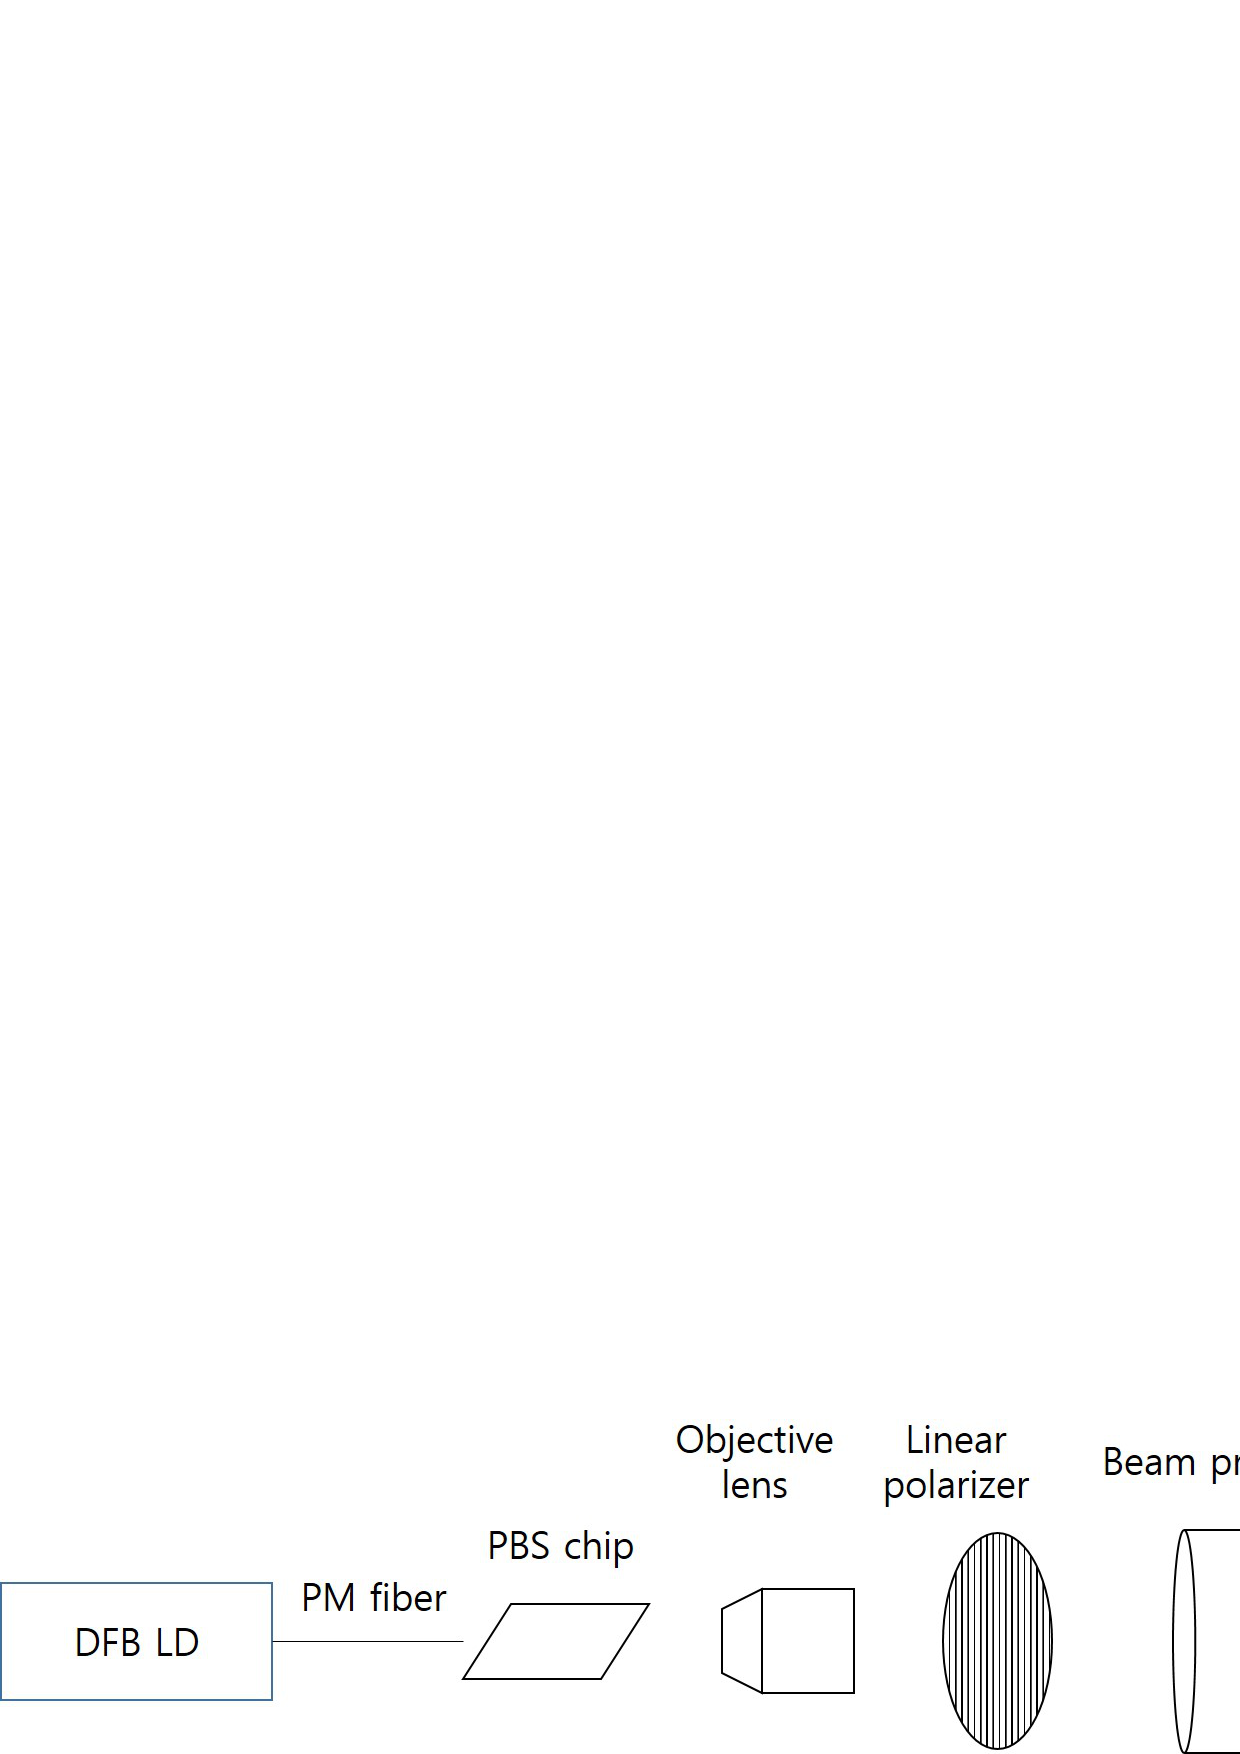
\includegraphics[width=13cm]{./setup.pdf}
  \caption{Schematic of the setup measuring PER of PBS chip. Obliquely polarized light is incident on the chip via PMF. The linear polarizer filters out the transmitted light to either H- or V-polarization, and the beam profiler measures the output power ratio of each waveguide.}
  \label{fig:setup}
\end{figure}
Output of a 780 nm distributed fee dBack LD was delivered to the PBS chip through a polarization-maintaining fiber (PMF) whose slow axis is aligned obliquely so that incident light contains both H- and V-polarization.
The output light from the chip was expanded through an objective lens and observed using a beam profiler (Ophir Optronics Spiricon SP503).
As the input polarization is neither H nor V, output light has both the polarizations.
In order to evaluate polarization extinction ratio (PER), a linear polarizer (LP) was placed between the objective lens and beam profiler.
If the transmission axis of the LP is vertical, only V-polarized light is considered to be incident on the beam profiler since the LP filters out the H-polarized light with high PER exceeding 30 dB.
This method is based on the assumption that rotation of polarization does not occur for both H- and V-polarized lights.
With polarization rotation in the PBS chip, PER would be deteriorated when measured after the chip is fabricated to PBS module that does not contain LP.
As will be discussed later, however, PBS module does not show any drop of PER, which suggests the validity of the assumption.

% PMF의 광축을 약 45도 정도 기울어지도록 설치한 후 칩에 정렬하여 빛을 입사시켰다.
%Laser output was launched on the chip through PMF whose optic axis was inclined by 45$^\circ$.
% 칩을 통과한 빛에는 H와 V 편광이 섞여있으며, 대물렌즈를 거쳐서 나오는 빛을 선형 편광판을 이용하여 측정하고자 하는 편광만을 걸러낸 후 빔프로파일러를 이용하여 출력 도파로로부터의 빛의 세기를 측정하였다.
% The light passing through the chip, whose polarization was mixed with H and V direction, was focused by an objective lens and filtered using a linear polarizer to either H or V polarized light.
PER was obtained by measuring the intensity from the output waveguides using a beam profiler while the current of the micro-heater was adjusted so that PER of PBS could be maximized.

% PBS 칩은 복굴절 도파로의 길이에 따라 다른 편광소광비 특성을 보였다.
The PBS chip showed different PER characteristics depending on the length of the birefringent waveguide (BRW) as shown in Fig. \ref{fig:BRW-PER}.
\begin{figure}
  \centering
  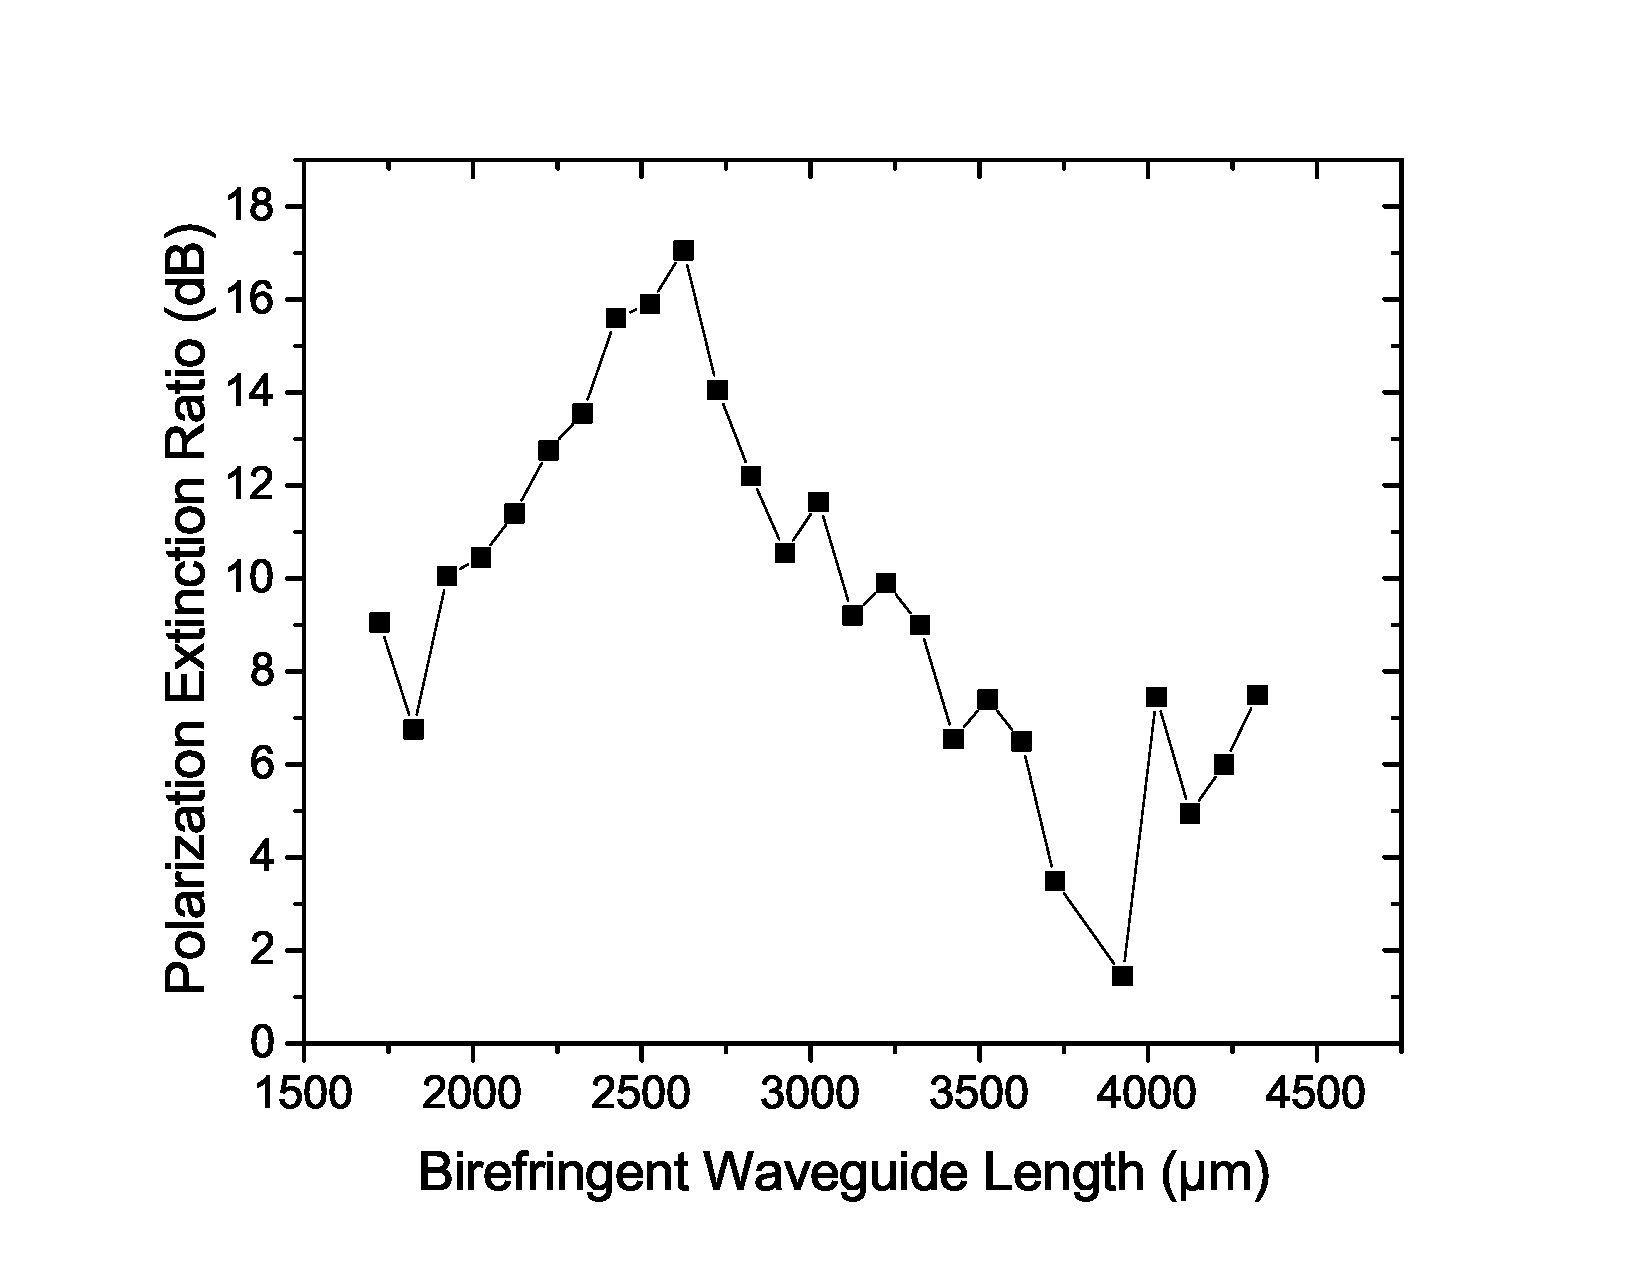
\includegraphics[width=7cm]{./BRWPER}
  \caption{Measured result of PER with birefringent waveguide length. Maximum PER of 17.1 dB was obtained when the BRW length is 2624 $\mu$m.}
  \label{fig:BRW-PER}
\end{figure}
% 최대의 편광소광비가 얻어지는 조건의 복굴절 도파로 길이는 약 ___ um 정도로, 이 길이에서 H와 V 간에 180도 위상차가 발생한다.
Maximum PER is 17.1 dB  if the length of BRW is 2624 $\mu$m.
 %where H- and V- polarization show phase difference of 180$^\circ$.
From this result, the birefringence of the BRW is estimated as 1.5$\times 10^{-4}$ that is similar to that reported in Ref. \cite{Hashizume:2015ta}.

% 본 연구에서 제작한 칩에서는 히터를 동작시켜야만 편광이 분리되었다.


\subsection{Half-Wave Plate Film}
% 제작된 반파장판 필름의 retardance를 polarimeter에 의한 편광 상태 측정을 통해서 조사하였다.
% Retardance of the waveplate fabricated was measured using polarimeter (Thorlabs PAX5720IR1) and linearly polarized laser output.
The optical output of the LD  was collimated and converted to D-polarized light by using a linear polarizer, and was transmitted through the waveplate film.
The resultant polarization state of the light was measured using a polarimeter (Thorlabs PAX5720IR1).
% D 방향의 편광을 입사시켰을 때 투과되어 나오는 빛의 편광을 폴라리미터로 관찰하여 H 또는 V 편광이 나오는 부분을 1.5mm X 1mm로 잘라내에 패키징에 사용할 필름 조각을 선별하였다.
% 앞의 공정 조건이 반파장 부근의 retardance를 주었으나 필름의 각 위치별로 retardance와 광축 방향의 편차가 존재해서 실제 모듈에 사용하기 위해서는 반파장 조건이 잘 맞는 부분을 골라야 했다.
While the film exhibited spatial variation in retardance and direction of the optical axis, some areas of the film were measured to be suitable for use in PBS.
Part of the film converting D(A)-polarization to H(V)-polarization was cut out into a size of 1.5 mm $\times$ 1.0 mm for being inserted into the groove of the PBS chip.
%Some parts satisfying both the conditions of 180$^\circ$-retardance were found in the film.
%But the film showed a spatial variation, and therefore
%However, since there was a spatial variation in the retardance of the film, the parts satisfying the half-wavelength condition were selected through measurement and cut out into a size of 1 mm $\times$ 1.5 mm for packaging.
% 다음 그림은 필름에 입사되는 빛의 편광과 통과된 후의 빛의 편광을 측정한 결과이다.
%Figure \ref{fig:Pol} shows the measured polarization state before and after the transmission through the waveplate film.
% 45도의 선형 편광이 수평이 되는 것을 확인할 수 있었다.
%It was confirmed that D-polarized incident light was converted to \underline{V}-polarized light through analysis using a polarimeter.
% 위의 그림에서와 같이 좋은 특성을 보이는 부분을 1.5mm X 1mm로 잘라내었다.
% 절단된 필름은 훔에 삽입되는데, 절단 과정이나 삽입 과정에서 광축이 틀어질 수 있으며 이는 소광비에 영향을 줄 수 있다. 그 영향을 보여주는 시뮬레이션 결과가 다음 그림에 나타나 있다.
% \begin{figure}
%   %\includegraphics{/path/to/figure}
%   \caption{}
%   \label{fig:Pol}
% \end{figure}
% 22.5도를 정확히 맞추지 못할 경우 최종적으로 편광 소광비에 어떤 영향을 주는지 계산해 본 결과는 다음 그림과 같다.

The direction of the optic axis may have a slight offset after the cutting  or  insertion process.
Figure \ref{fig:angle_offset} shows how PER is affected by the offset angle from 22.5$^\circ$.
\begin{figure}
  \centering
  \includegraphics[width=8cm]{./offset_angle}
  \caption{PER (left axis) and its degradation (right axis) as functions of the offset angle of HWP inserted in PBS for DA-polarization. PER decreases with the offset angle, and the degradation is the larger when PER at exact angle is the higher.}
  \label{fig:angle_offset}
\end{figure}
% offset 각도가 커짐에 따라 PER이 나빠지는 것을 볼 수 있다.
PER gets degraded with the increase of the offset angle.
The offset angle prevents the 45$^\circ$ polarized incident light from being converted into purely V-or H-polarized light, thus reducing PER of the PBS behind the HWP.
%The extent of the degradation is larger when PER at exact angle is higher.
% offset angle은 45도 편광을 완전한 V 또는 H 편광으로 만들 수 없도록 하므로 반파장판 뒤에 오는 PBS의 편광 소광비를 떨어뜨리는 역할을 한다.
% PER의 열화는 최종적으로는 QKD 시스템의 QBER을 나쁘게 해서 key rate를 떨어뜨리는 효과를 불러온다.
%The deterioration of the PER eventually leads to increase of quantum bit error rate (QBER) of the QKD system, thereby lowers the key rate.
% 그러나 그림에서 볼 수 있는 것처럼 0도에서 2도 정도까지는 PER의 열화가 그리 크지 않아서 약간의 각도의 부정확성이 전체적인 performance에는 크게 영향을 주지는 않을 것임을 알 수 있다.
However, Fig. \ref{fig:angle_offset} suggests that the drop of PER is not so large within  offset angle of 2$^\circ$, and  a slight inaccuracy in the angle  will not significantly affect the overall performance.
In our study, the film cutting or treatment could be accomplished without any specialized equipment within that precision.
%to keep the direction of the optic axis of the film within that precision was not difficult without any specialized equipment for film cutting or treatment.

\subsection{PBS Module}
% 모듈의 편광 분리 특성은 편광조절기로 입력광의 편광을 바꿔가면서 얻어지는 출력광들의 세기의 비가 최대가 되도록 해서 편광소광비를 구하여 평가하였다.
The polarization-splitting characteristics of the module were evaluated by receiving light from sender (Alice) of free-space QKD test-bed and measuring the optical powers from the four PMFs of the PBS module, as shown in Fig. \ref{fig:meas_setup}(a).
%determining PER when the intensity ratio of the output light was maximized by manipulating a polarization controller (PC) connected with the input fiber of the module.
% 실제로 입력광의 편광이 어떤 상태인지 알 수 없었으므로 이렇게 구한 편광 소광비가 올바른 값인지 확신할 수 없다.
At the chip temperature of 21$^\circ$C and current of the micro-heater of 29 mA, the module shows PER of 22.4 dB in separating H/V polarizations, and 17.6 dB for D/A polarizations.
This is better than the result obtained from PBS chip measurement.
It is owing to both temperature optimization and better fiber-chip alignment in the module.
In chip measurement, it is difficult to align the fiber with right angle to the facet of the chip.
Therefore stray light is apt to occur and part of the can be coupled to unwanted output waveguide, worsening PER than the MZI can provide.
On the other hand, the V-groove block for fiber-pigtail in module fabrication helps normal incidence of light and thus minimizes stray light.

While this polarization-splitting capability is used before single-photon detectors by receiver (Bob), the module can also be used as PBC for combining four polarization states by Alice.
Since common SMF is used as the output port in the module, there is no need to perform precise alignment so that the four polarized lights propagate along the identical path in the free space.
%As the module emits light through one SMF, there is no need to precisely align the four outputs of LDs so that they travel along the identical path in free space.
If four PMF-pigtailed LDs are connected to the PMFs of the PBS module, output polarizations of the LDs are converted to H-V-H-V  by the PMFs of the module, and converted to  H-V-D-A  by the HWP film in the PBS chip.

The performance of the module as a PBC was assessed by connecting the SMF of the module with a polarimeter via a polarization controller (PC) that is configured to compensates the polarization distortion occurring in the SMF, as shown in Fig. \ref{fig:meas_setup}(b).
If the module is not properly fabricated, no configuration of the PC can restore the four LDs' output to their original states simultaneously.
The four states of the polarization measured is shown in Fig. \ref{fig:meas_setup}(c).
\begin{figure}
  \centering
  \includegraphics[height=7.5cm]{meas_setup}
  \caption{(a) Setup for measuring PER of the PBS module using Alice part of a free-space QKD test-bed. PBS module splits the input light according to its polarization, and power ratio between the outputs are obtained by measured optical powers.  (b) Setup for characterizing the module as a PBC. Output from the four LDs are combined in the module and emitted through the SMF. PC is configured to compensates all the polarization. The final polarization state  is observed by the polarimeter. (c) Measured polarization states of the PBS module output in (b) represented in Poincar\'{e} sphere.}
  \label{fig:meas_setup}
\end{figure}
Each output state is quite close to the four polarization states of H/V/D/A.
The minimum extinction ratio of the output was as large as 346:1.
The good performance of the module as a PBC suggests the exact retardance and optic-axis alignment of the HWP film.



Total optical  loss of the module was measured to be 7.7 dB including 3 dB splitting loss of Y-branch.
The fiber-chip coupling loss at both the facets was estimated to be 1.0 dB from additional experiment.
Therefore excess optical loss occurring in the chip is about 3.7 dB.
% PBS 모듈에서 광손실은 광섬유와의 결합 손실, 도파로 내에서의 radiation loss, 필름 삽입을 위한 홈에서 발생하는 손실을 들 수 있다.
This loss is mainly due to the groove for HWP film insertion.
Diffraction loss occurs at the waveguide gap caused by the groove, and it increases drastically with increasing gap width \cite{Inoue:1997es}.
Chipping that might occur on the edge of the diced groove surface can cause scattering loss \cite{Carpenter:2013fh}.
% 그것들 중 홈에서의 손실이 ___ dB로 추정되며 이것은 더 좁은 홈과 거기에 맞는 반파장판을 사용하면 줄일 수 있다.
% 30um로 홈을 줄이면 1.5 dB 정도의 손실을 줄일 수 있을 것으로 예상된다.
It is expected from a beam propagation method simulation that the loss will be decreased by about 1.5 dB if the width of the groove is reduced to 30 $\mu$m by developing thinner half-wave plate film.
The loss would be further reduced if groove-dicing process is optimized to suppress chipping.

% 그러나 추가의 실험을 통해서
\subsection{QKD Test}
%B84 테스트베드의 Bob 파트에 장착하여 key 전송 실험을 수행했다.
The free-space BB84 test was performed with the fabricated module replacing the four polarization splitting block on the Bob part of the test-bed, as shown in Fig. \ref{fig:testbed}.
\begin{figure}
  \centering
  \includegraphics[width=13cm]{testbed3.pdf}
  \caption{Setup for evaluating the integrated PBS module in the Bob part of a free-space QKD system. The module replaced one BS, one HWP, and two PBSes. Attn.: attenuator, DM: dichroic mirror, Sync. Laser: synchronization laser, M: mirror, Sync. Detector: synchronization detector, PC: polarization controller, SPD: single photon detector, FPGA: field-programmable gate array}
  \label{fig:testbed}
\end{figure}
%%% 수신부 테스트 조건 %%%
% 100MHz로 클럭을 발생시켰고, 두 개의 난수 발생기를 이용하여 네 개의 LD 중 하나로부터 빛을 100MHz의 주파수로 발생시켰다.
In the Alice part, two random number generators were used to choose the basis and binary data, and one of the four LDs emitted light accordingly under the clock rate of 100 MHz.
% LD로부터의 빛은 PBS, BS를 통해 동일한 경로가 되도록 했고, ND 필터로 펄스당 0.1개의 광자 레벨이 되도록 감쇄시켰다.
Collimated light from the four LDs transmitted  through the bulk optic PBS, BS, and HWP, and was finally attenuated to mean photon number of 0.1 per pulse by a neutral density filter.
LD signal with wavelength of 1550 nm was transmitted through dichroic mirror with quantum signal for synchronization of Alice and Bob.
% Bob 시스템에서는 collimation lens 를 통해 들어온 빛을 광섬유에 결합시켰고, 광섬유 편광조절기를 사용하여 편광 모듈의 칩으로 들어간 빛의 편광이 원래의 편광이 되도록 조절하였다.
In the Bob part, the light from Alice was  focused by lens and coupled to an SMF.
The SMF and our integrated PBS module was connected via a PC that could restore the polarization of the light entering the PBS chip to the original one that Alice sent.
% 편광 모듈의 출력 쪽 네 개의 광섬유는 각각 단일광자 검출기에 연결하였다.
The each PMF on the output side of the PBS module was connected to a single photon detector.
% 테스트베드 구동 결과 overall QBER은 2.8%, sifted key rate 은 ___ kbps가 얻어졌다.
As a result of the test-bed operation, overall QBER was 2.81\% and sifted key rate were 415 kbps, as shown in Fig. \ref{fig:QKD_result}.
\begin{figure}[ht]
  \centering
  \subfigure[]{\includegraphics[height=5.6cm]{key_rate}}
  \subfigure[]{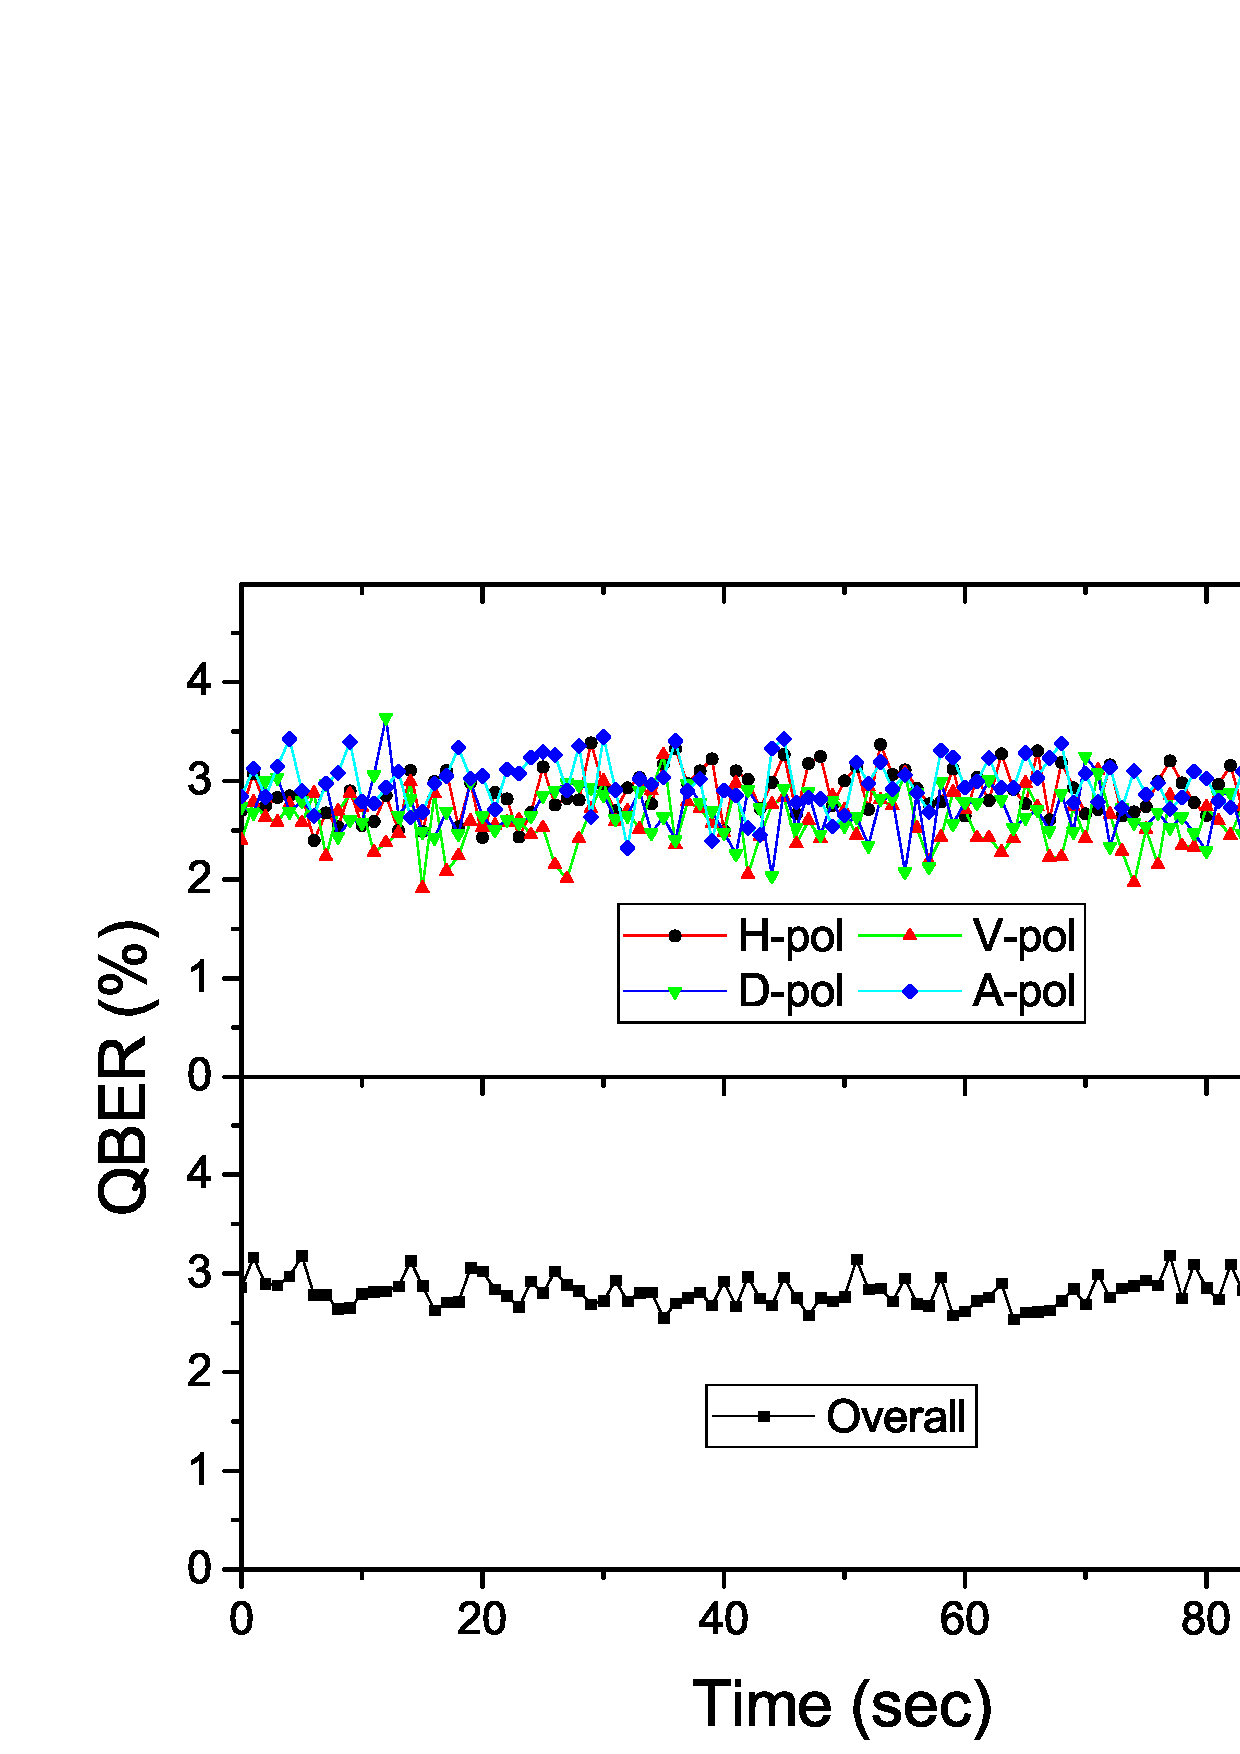
\includegraphics[height=5.2cm]{QBER}}
  \caption{Test result for the PBS module in a free-space BB84 protocol test-bed. (a) raw key rate and sifted key rate for 100 sec and (b) QBER of four channels and overall QBER for 100 sec.}
  \label{fig:QKD_result}
\end{figure}
% 편광 모듈 대신 벌크 옵틱스를 사용했을 때는 QBER과 sifted key rate은 각각 __%와 ___kbps였다.
When bulk optic components were used instead of our PBS module, QBER and sifted key rate were measured to be 0.69\% and 1.56 Mbps, respectively.
% 두 경우의 차이는 대부분 편광 모듈에서의 손실에서 기인한다고 할 수 있다.
The difference between the two cases is attributable to relatively high optical loss and low PER of our PBS module compared to the bulk optic components.
% ___ dB의 손실은 이상적으로는 ___%의 QBER을 유발한다.
%In ideal case optical loss of \underline{23903} dB corresponds to QBER of \underline{2392}\%.
MZI-based PBS chips for 1.55 $\mu$m wavelength generally show better PER than the chip developed in this work \cite{Hashizume:2015ta}.
MZI works on the basis of phase relation that is determined by physical lengths of the two arms.
As the operation wavelength in this study is about half of that of optical telecommunication application, the performance of the MZI structure is more sensitive to small change in optical path length, and design optimization is more difficult.
Thus PER can be further improved by either optimizing the chip design with finer length variation or adopting smaller birefringence in BRW.


\section{Conclusion}
% 780 nm 파장 대역에서 편광 기반의 BB84 프로토콜 양자암호통신을 위해  HVDA의 네 편광을 분리 및 결합하는 집적형 편광분배기 모듈을 개발하였다.
Waveguide-based integrated PBS module was developed for the first time that could separate the H/V/D/A polarizations for polarization-based BB84 QKD protocol in the 780 nm wavelength band.
% CW 레이저를 이용하여 측정한 편광 소광비는 최소 ___ dB를 보였고 제작된 모듈을 무선 양자암호 테스트베드에 장착하여 테스트 한 결과 sifted key rate는 ___kbps, QBER은 ___% 였으므로 보안 통신을 할 수 있는 충분한 성능을 확인하였다.
The PBS module showed minimum PER of 17.6 dB.
When the module was tested in Bob part of a free-space QKD test-bed, the measured sifted key rate was 415 kbps and QBER was 2.81\% at clock rate of 100 MHz, respectively.
% 벌크 옵틱스 기반으로 구성한 편광분할을 했을 때의 sifted key rate와 QBER은 각각 ___와 ___였으며 두 경우의 차이는 주로 광모듈 내의 광손실에서 기인한 것으로 생각된다.



\section*{Funding}
This work was supported by Electronics and Telecommunications Research Institute (ETRI) grant funded by the Korean government. [Development of transceiver components and system control technologies for the polarization based free space quantum key distribution]
%\section*{Acknowledgments}
\end{document}
